%!TeX program = xelatex
\documentclass{SYSUReport}
\usepackage{amsmath}
\usepackage{amssymb}
\usepackage{tikz}
\usepackage{adjustbox}
\usepackage{booktabs}
\usepackage{multirow}
\usepackage{graphicx}
\usepackage{longtable}
\usepackage{listings}
\usepackage{xcolor}
\usepackage{hyperref}

\lstdefinestyle{mystyle}{
    backgroundcolor=\color{gray!10},
    basicstyle=\ttfamily\small,
    keywordstyle=\color{blue!70!black},
    commentstyle=\color{green!40!black},
    stringstyle=\color{purple!60!black},
    numbers=left,
    numberstyle=\tiny\color{gray},
    frame=single,
    breaklines=true,
    captionpos=b
}
\lstset{style=mystyle}

\headl{24347014 陈泳强}
\headr{实验五：联邦学习框架调研与复现}
\lessonTitle{数据安全和隐私保护}
\reportTitle{实验五：联邦学习框架调研与复现}
\stuname{陈泳强}
\stuid{24347014}
\inst{网络空间安全学院}
\major{网络空间安全}
\date{2026 年 11 月 26 日}

\begin{document}

\cover
\thispagestyle{empty}
\clearpage

\tableofcontents
\clearpage

\pagenumbering{arabic}
\setcounter{page}{1}

% =========================================================
\section{实验要求与环境}

\subsection{实验要求}

本实验调研并复现开源联邦学习框架，完成横向联邦图像分类实验，理解客户端本地训练与模型聚合，比较 IID 与标签偏斜两种数据分布下的训练效果，并分析联邦学习的隐私保护边界。具体包括：选择并安装一个开源联邦学习框架；使用 MNIST 与小型全连接网络，按每类 500 张（共 5000 张、seed=42）构造近似 IID 与标签偏斜两套划分；1 个服务器 + 5 个客户端、FedAvg、10 轮、每轮全参与、每客户端本地遍历 1 次，SGD（lr=0.01、batch=32、无动量、无权重衰减）；记录初始模型与每轮全局模型在官方测试集上的准确率与逐样本平均损失，绘制曲线并比较耗时；在标签偏斜下做 5 个客户端独立本地训练的对照；分析“数据不出本地”与隐私安全的关系。

\textbf{选做完成情况：}本次完成了拓展任务——3 客户端整数向量求和的成对随机掩码安全聚合演示，见第 \ref{sec:secure-agg} 节。

\subsection{实验环境}

\begin{itemize}
  \item 操作系统：Windows 11，终端 Git Bash（MINGW64）
  \item Python 环境：conda 环境 \texttt{he}，Python 3.12.15
  \item 依赖库：\texttt{flwr[simulation]} 1.43.0（含 ray 2.55.1）、\texttt{torch} 2.15.0+cpu、\texttt{torchvision} 0.29.2+cpu、\texttt{matplotlib} 3.11.2
  \item 报告编译：Overleaf + XeLaTeX，模板 \texttt{SYSUReport.cls}
  \item 代码仓库：\url{https://github.com/Skylarkyq06/research-tools-weeks}，实验五代码位于 \texttt{experiment5/}
\end{itemize}

\subsection{代码与数据目录}

\begin{lstlisting}[language=bash, caption={实验五代码与数据目录}]
experiment5/
|-- __init__.py
|-- src/
|   |-- __init__.py
|   |-- model.py            # MLP 定义、参数序列化、评估
|   |-- data.py             # MNIST 抽取、IID 与标签偏斜划分
|   |-- client.py           # Flower NumPyClient
|   |-- strategy.py         # LoggingFedAvg + 指标写入 CSV
|   |-- run_fed.py          # IID / Skew FedAvg 启动脚本
|   |-- local_baseline.py   # 本地独立训练对照
|   `-- plot_curves.py      # 绘制训练曲线
|-- tests/
|   |-- test_data.py        # 划分样本数、类别分布、互不重复验证
|   `-- test_model.py       # 前向形状、参数序列化验证
|-- results/                # CSV 与 JSON，报告数字均来源于此
`-- report/                 # main.tex、SYSUReport.cls、figures/
\end{lstlisting}

% =========================================================
\section{联邦学习框架调研}

\subsection{框架选型}

题目建议优先调研 MindSpore Federated。但 MindSpore Federated 官方文档明确其联邦学习功能目前仅支持 Linux 与 Android 平台，Windows 不在支持范围内，无法在当前 Windows 11 + Python 3.12 环境下完成安装与实验。题目允许“也可选用 Flower 等”，因此选用 \textbf{Flower}。

Flower 要求 Python $\geq$ 3.11，Python 3.12 已获正式支持，\texttt{pip install "flwr[simulation]"} 即可安装，且内置 FedAvg 等策略与 NumPyClient 接口，与本实验需求完全匹配。

\subsection{Flower 架构与接口}

Flower 采用客户端—服务器架构：

\begin{itemize}
  \item \textbf{Server}：由 \texttt{Strategy} 决定客户端选择与参数聚合方式。本实验使用 \texttt{FedAvg} 并派生 \texttt{LoggingFedAvg} 记录指标。
  \item \textbf{Client}：实现 \texttt{fit}（本地训练并返回参数和样本数）与 \texttt{evaluate}（本地评估）两个接口，通过 gRPC 与 Server 通信。
  \item \textbf{Simulation}：通过 \texttt{flwr.simulation.run\_simulation} 在单机上用 Ray 拉起 1 个 Server 与 $N$ 个 Client actor，无需真实网络。
\end{itemize}

内置算法包括 FedAvg、FedProx、FedOpt 等；通信方式为 gRPC，支持 TLS 与安全聚合（SecAgg）扩展。本实验示例来源为 Flower 官方 PyTorch quickstart（\url{https://flower.ai/docs/framework/tutorial-quickstart-pytorch.html}）。

\begin{figure}[htbp]
  \centering
  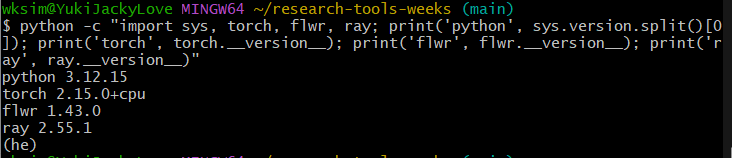
\includegraphics[width=0.85\textwidth]{figures/fig_env.png}
  \caption{实验环境版本（Python、torch、flwr、ray）}
\end{figure}

% =========================================================
\section{实验原理}

\subsection{FedAvg 聚合公式}

横向联邦学习中各客户端特征与标签空间相同、样本不同。客户端基于服务器下发的全局模型做本地训练并上传参数，服务器聚合后生成新全局模型。FedAvg 按客户端样本数加权平均：
\begin{equation}
w_{t+1} = \sum_{k=1}^{K}\frac{n_k}{\sum_{j=1}^{K}n_j}\, w_{t+1}^{(k)},
\end{equation}
其中 $K$ 为客户端数，$t$ 为轮次，$n_k$ 为客户端 $k$ 的样本数，$w_{t+1}^{(k)}$ 为其本地训练后的参数。本实验 $K=5$，各客户端 $n_k=1000$，加权平均退化为算术平均，但实现上仍按一般公式加权。

\subsection{近似 IID 与标签偏斜}

近似 IID 划分使各客户端类别比例相同：每个客户端都含类别 0 到 9，每类 100 张，共 1000 张。标签偏斜划分使客户端仅持有部分类别：客户端 $k$ 持有类别 $2k$ 与 $2k+1$，每类 500 张，共 1000 张，属于非独立同分布（Non-IID）情形。两套划分使用完全相同的 5000 个样本，只改变分组方式。

% =========================================================
\section{系统流程}

\subsection{信息传递流程}

每轮的信息传递如下：Server 将当前全局参数 $w_t$ 下发给全部 5 个客户端；每个客户端用本地数据做 1 个 epoch 的 SGD，得到 $w_{t+1}^{(k)}$ 并连同样本数 $n_k$ 上传；Server 按样本数加权聚合得到 $w_{t+1}$；随后在官方测试集上评估并写入 CSV；进入下一轮，共 10 轮。

\begin{center}
\begin{tikzpicture}[scale=0.9, every node/.style={font=\small}]
  \node[draw, rounded corners, fill=blue!10, minimum width=4.5cm] (S) at (4,3.5) {\textbf{Server}（全局参数 $w_t$）};
  \node[draw, rounded corners, fill=green!10, minimum width=4.5cm] (C) at (4,0) {\textbf{5 个客户端}（本地数据 $D_1,\dots,D_5$）};
  \coordinate (L1) at (0.8,3.5);
  \coordinate (L2) at (0.8,0);
  \coordinate (R1) at (7.2,3.5);
  \coordinate (R2) at (7.2,0);
  \draw[->, thick, blue!70] (S.west) -- (L1) -- (L2) -- (C.west);
  \draw[->, thick, red!70] (C.east) -- (R2) -- (R1) -- (S.east);
  \node[left, font=\scriptsize, align=center] at (0.8,1.75) {1. 下发\\$w_t$};
  \node[right, font=\scriptsize, align=center] at (7.2,1.75) {2. 上传\\$w_{t+1}^{(k)}, n_k$};
  \node[align=center, font=\small] at (4,1.75) {3. Server 按 $n_k$ 加权聚合\\4. 在官方测试集评估并写 CSV};
\end{tikzpicture}
\end{center}

\subsection{训练设置}

10 轮，每轮全部 5 个客户端参与，每客户端本地遍历数据 1 次；交叉熵损失；SGD，无动量、无权重衰减；学习率 0.01；批量大小 32。两组使用相同的初始参数（seed=42）、相同网络结构和预处理（ToTensor + Normalize(0.1307, 0.3081)）。测试集为官方 10000 张，不参与训练。

% =========================================================
\section{数据准备与客户端划分}

\subsection{数据抽取}

从 MNIST 官方训练集中每类随机抽取 500 张，共 5000 张，随机种子 42。两套划分使用完全相同的 5000 个样本，同一套内各客户端样本互不重复。

\subsection{两套划分}

\begin{table}[h]
\centering
\caption{两套划分的客户端数据组成}
\begin{tabular}{lcc}
\toprule
划分方式 & 各客户端数据组成 & 每客户端样本数 \\
\midrule
近似 IID & 均含类别 0--9，每类 100 张 & 1000 \\
标签偏斜 & 依次持有 0/1、2/3、4/5、6/7、8/9 类，每类 500 张 & 1000 \\
\bottomrule
\end{tabular}
\end{table}

\subsection{划分验证}

\texttt{experiment5/tests/test\_data.py} 检查了四项：base 样本 5000 且唯一、每类 500；两套划分并集均等于 base 的 5000 个索引；每个客户端 1000 张；IID 每类 100、Skew 客户端 $k$ 只有类别 $2k$ 和 $2k+1$ 各 500。全部断言通过，输出见下图。

\begin{figure}[h]
\centering
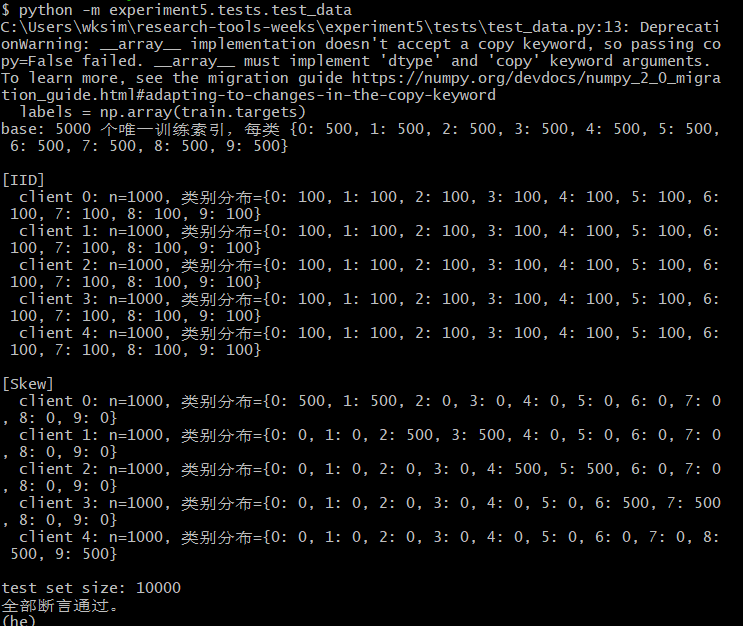
\includegraphics[width=0.92\textwidth]{figures/fig_data_split.png}
\caption{数据划分验证输出（IID 每客户端每类 100；Skew 客户端 0 只有类别 0/1 各 500，依此类推）}
\label{fig:data-split}
\end{figure}

% =========================================================
\section{关键代码解释}

\subsection{模型}

小型全连接网络：784 $\to$ 128 $\to$ 10，ReLU 激活，参数量 101770。

\begin{lstlisting}[language=Python, caption={MLP 模型定义（model.py）}]
class MLP(nn.Module):
    def __init__(self):
        super().__init__()
        self.fc1 = nn.Linear(784, 128)
        self.relu = nn.ReLU()
        self.fc2 = nn.Linear(128, 10)

    def forward(self, x):
        x = x.view(x.size(0), -1)
        x = self.relu(self.fc1(x))
        return self.fc2(x)
\end{lstlisting}

\subsection{数据划分}

IID 划分：每类 500 张洗牌后均分 5 份，每客户端每类 100。标签偏斜：客户端 $k$ 直接取类别 $2k$、$2k+1$ 的全部样本。

\begin{lstlisting}[language=Python, caption={标签偏斜划分（data.py）}]
def split_skew(indices, labels):
    clients = [[] for _ in range(NUM_CLIENTS)]
    for k in range(NUM_CLIENTS):
        for c in (2 * k, 2 * k + 1):
            clients[k].extend(indices[labels[indices] == c])
    return [np.sort(np.array(ci)) for ci in clients]
\end{lstlisting}

\subsection{Flower 客户端}

\texttt{FlowerClient.fit} 从服务器参数恢复模型，用 SGD（\texttt{lr=0.01, momentum=0, weight\_decay=0}）遍历本地数据 1 个 epoch，返回参数与样本数 $n_k$。洗牌种子由 \texttt{seed + round*100 + partition\_id} 决定，保证可复现。

\subsection{聚合策略}

\texttt{LoggingFedAvg} 继承 \texttt{FedAvg}，提供 \texttt{fit\_metrics\_aggregation\_fn} 按样本数加权聚合本地损失；\texttt{aggregate\_fit} 在聚合后调用 \texttt{evaluate\_fn} 在官方测试集上评估全局模型并写 CSV。

\begin{lstlisting}[language=Python, caption={聚合与评估（strategy.py）}]
def weighted_average(metrics):
    total = sum(num for num, _ in metrics)
    loss = sum(num * m["train_loss"] for num, m in metrics) / total
    return {"train_loss": loss}

def aggregate_fit(self, server_round, results, failures):
    params, metrics = super().aggregate_fit(server_round, results, failures)
    train_loss = None if not metrics else metrics.get("train_loss")
    test_loss, test_acc = None, None
    if params is not None:
        ndarrays = parameters_to_ndarrays(params)
        test_loss, eval_metrics = self.evaluate_fn(server_round, ndarrays, {})
        test_acc = eval_metrics.get("accuracy")
    # 写 CSV：round, test_loss, test_accuracy, train_loss, round_time_sec
    return params, metrics
\end{lstlisting}

% =========================================================
\section{训练结果与曲线}

\subsection{初始模型与每轮指标}

初始全局模型在测试集上准确率 0.1078、损失 2.2840，接近随机猜测，符合预期。两套划分每轮全局模型在官方测试集上的指标如下。

\begin{table}[h]
\centering
\caption{每轮全局模型测试准确率（初始模型 0.1078）}
\begin{tabular}{cccc}
\toprule
轮次 & IID 准确率 & 标签偏斜准确率 \\
\midrule
1  & 0.6526 & 0.3972 \\
2  & 0.7622 & 0.6274 \\
3  & 0.8089 & 0.7148 \\
4  & 0.8317 & 0.7489 \\
5  & 0.8480 & 0.7691 \\
6  & 0.8575 & 0.7861 \\
7  & 0.8650 & 0.7974 \\
8  & 0.8711 & 0.8044 \\
9  & 0.8757 & 0.8095 \\
10 & 0.8799 & 0.8129 \\
\bottomrule
\end{tabular}
\end{table}

IID 第 10 轮准确率 0.8799、测试损失 0.4736；标签偏斜第 10 轮 0.8129、0.8977。值得注意的是：标签偏斜的客户端本地训练损失降到 0.1883，远低于 IID 的 0.5025，但全局测试损失反而更高。这说明各客户端只拟合自己持有的 2 个类别，本地损失很低，聚合后的全局模型对其余 8 类的判别能力不足，是 Non-IID 下“本地过拟合、全局泛化差”的典型表现。

\subsection{训练曲线}

\begin{figure}[h]
\centering
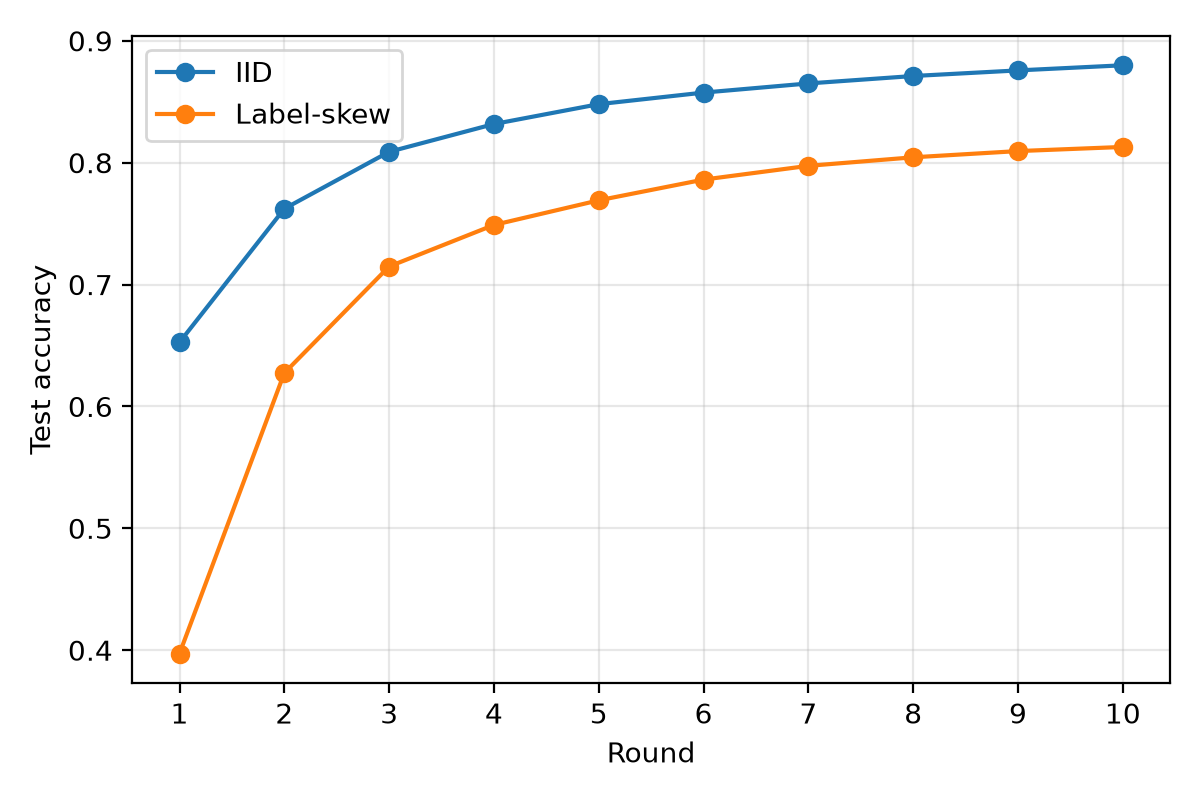
\includegraphics[width=0.75\textwidth]{figures/fig_accuracy.png}
\caption{测试准确率随轮次变化}
\label{fig:acc}
\end{figure}

\begin{figure}[h]
\centering
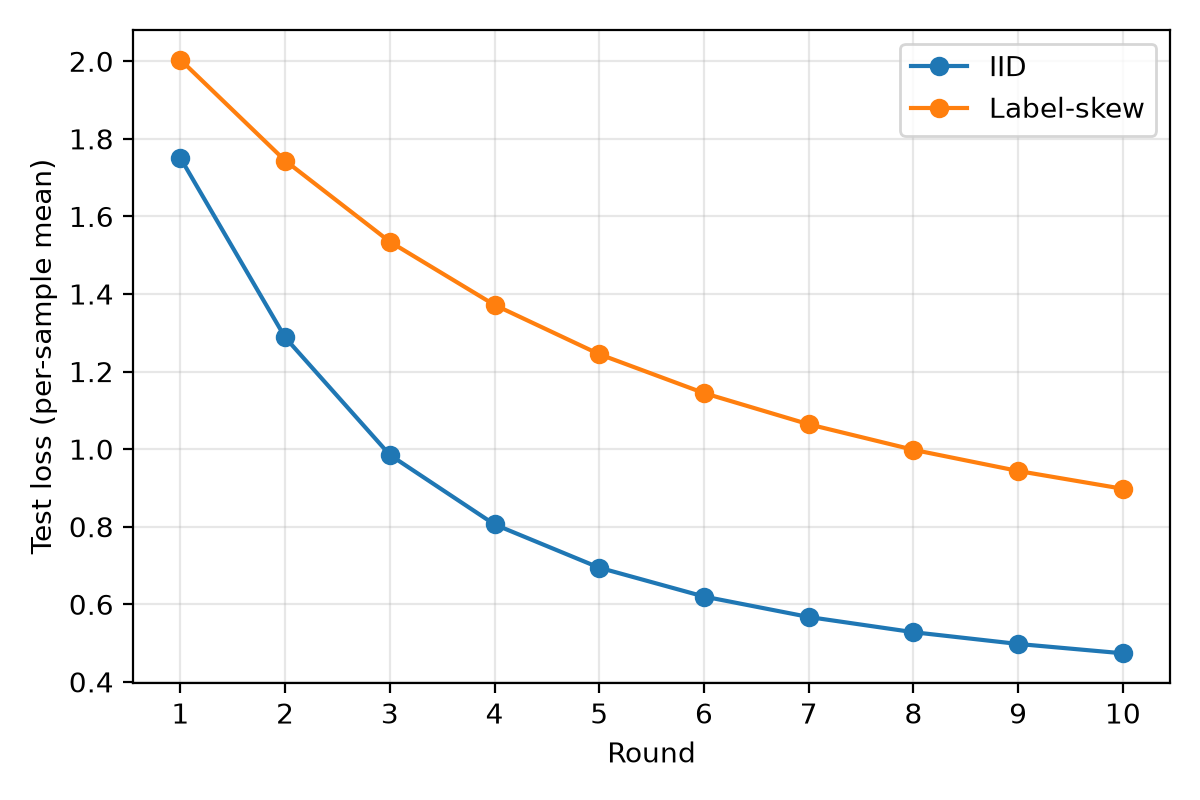
\includegraphics[width=0.75\textwidth]{figures/fig_test_loss.png}
\caption{测试集逐样本平均损失随轮次变化}
\label{fig:test-loss}
\end{figure}

\begin{figure}[h]
\centering
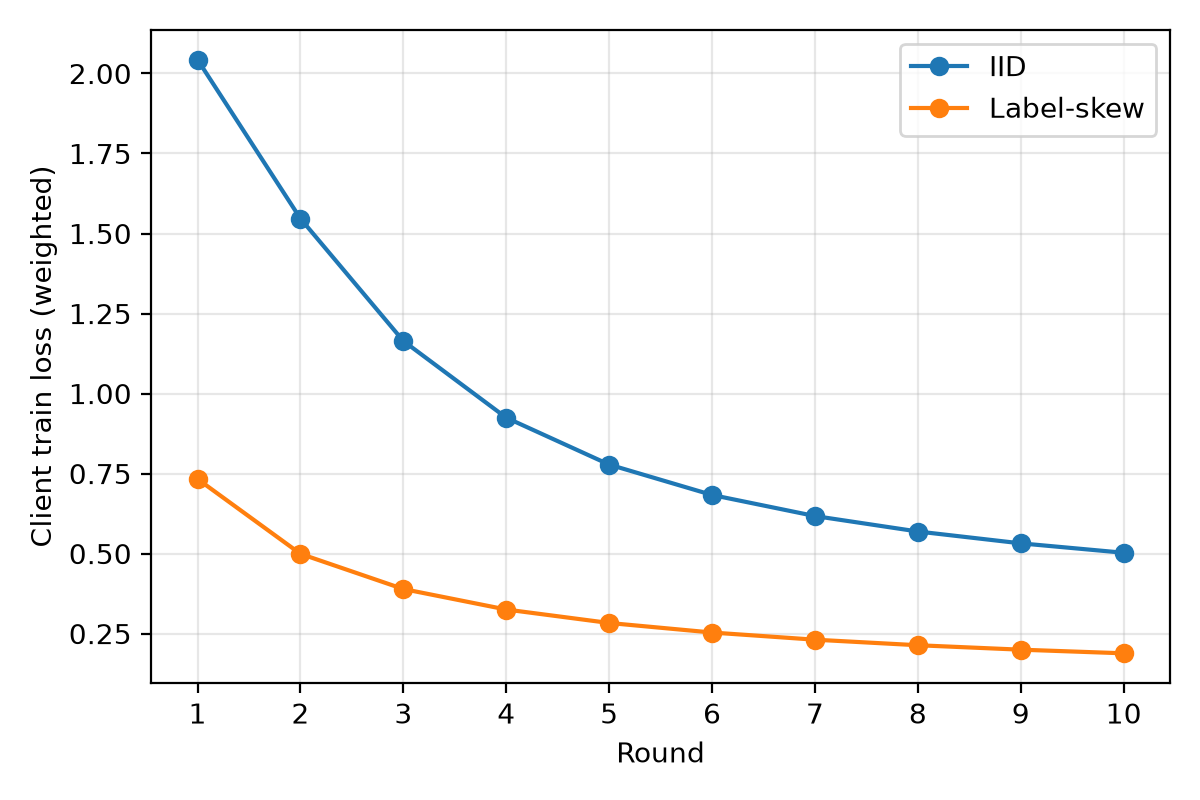
\includegraphics[width=0.75\textwidth]{figures/fig_train_loss.png}
\caption{客户端本地训练损失（按样本数加权）随轮次变化}
\label{fig:train-loss}
\end{figure}

\begin{figure}[h]
\centering
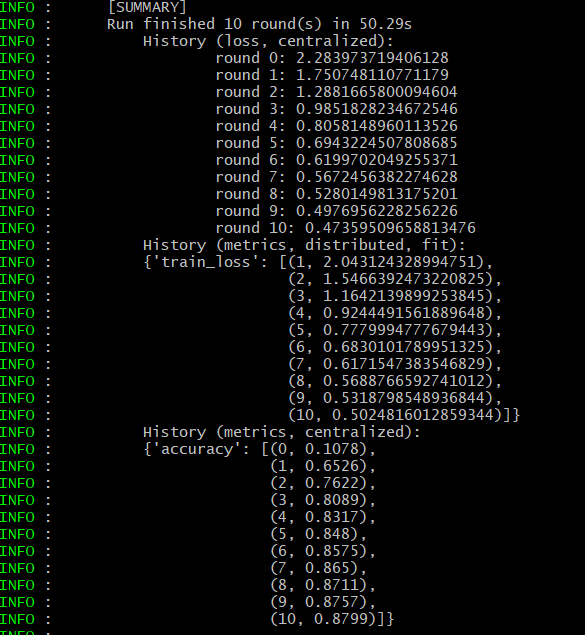
\includegraphics[width=0.92\textwidth]{figures/fig_iid_summary.png}
\caption{IID 运行日志 SUMMARY 段（10 轮 centralized loss 与 accuracy）}
\label{fig:iid-summary}
\end{figure}

\begin{figure}[h]
\centering
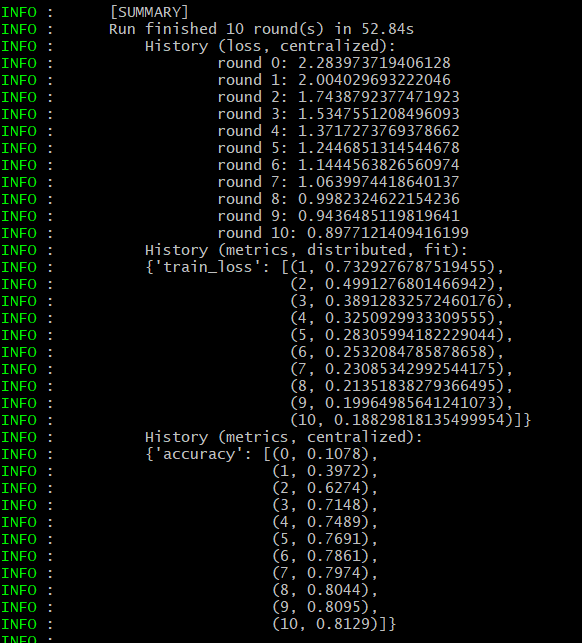
\includegraphics[width=0.92\textwidth]{figures/fig_skew_summary.png}
\caption{标签偏斜运行日志 SUMMARY 段}
\label{fig:skew-summary}
\end{figure}

% =========================================================
\section{对照实验与结果分析}

\subsection{本地独立训练}

在标签偏斜划分下，5 个客户端从与联邦实验相同的初始参数（seed=42）出发，仅用各自数据连续训练 10 个 epoch，不交换参数。与联邦实验中每客户端累计遍历 10 次的数据量一致；其余训练设置（SGD、lr=0.01、batch=32、无动量、无权重衰减）保持不变。

\begin{table}[h]
\centering
\caption{第 10 轮全局模型与本地独立模型对比}
\begin{tabular}{lcc}
\toprule
模型 & 测试准确率 & 测试损失 \\
\midrule
联邦 IID 第 10 轮全局模型 & 0.8799 & 0.4736 \\
联邦标签偏斜第 10 轮全局模型 & 0.8129 & 0.8977 \\
\midrule
本地 client 0（类别 0/1） & 0.2112 & 5.1817 \\
本地 client 1（类别 2/3） & 0.1969 & 6.0237 \\
本地 client 2（类别 4/5） & 0.1853 & 7.1703 \\
本地 client 3（类别 6/7） & 0.1969 & 5.9956 \\
本地 client 4（类别 8/9） & 0.1915 & 6.2176 \\
\bottomrule
\end{tabular}
\end{table}

\begin{figure}[h]
\centering
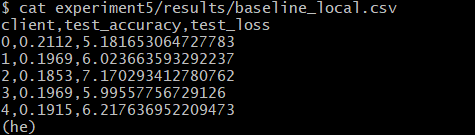
\includegraphics[width=0.85\textwidth]{figures/fig_baseline.png}
\caption{本地独立训练对照结果}
\label{fig:baseline}
\end{figure}

\subsection{结果对比}

本地模型准确率集中在 0.1853--0.2112，接近“只认识 2 个类别”的理论上限（约 0.2），测试损失高达 5--7，说明其对未见类别输出置信度错误且惩罚很重。联邦标签偏斜模型虽然也只在每客户端见过 2 类，但通过聚合获得了全部 10 类的信息，第 10 轮准确率达到 0.8129，比最好的本地模型高约 0.60。这直接说明联邦协作的价值：单个客户端的数据不足以训练可用分类器，参数聚合把分散的类别信息汇集到全局模型。

\subsection{数据分布的影响}

联邦标签偏斜模型仍低于 IID 模型约 0.067，说明数据分布对联邦训练有实质影响。标签偏斜下客户端本地目标与全局目标不一致，聚合参数在各类别间存在冲突，收敛更慢、最终精度更低。本实验不预设性能排序，以上结论均来自实际曲线与对照数字。

% =========================================================
\section{耗时}

统一计时口径为从 \texttt{run\_simulation} 调用开始到返回的墙钟时间，含 Ray 启动与客户端 actor 初始化，剔除 MNIST 下载与依赖安装时间。

\begin{table}[h]
\centering
\caption{两套划分训练耗时}
\begin{tabular}{lcc}
\toprule
划分 & Flower 内部计时 (s) & 墙钟计时 (s) \\
\midrule
IID & 50.29 & 54.57 \\
标签偏斜 & 52.84 & 56.89 \\
\bottomrule
\end{tabular}
\end{table}

两者耗时接近，说明在相同轮数与样本量下，数据分布本身不显著改变计算量；第 1 轮耗时明显偏高（约 17 s），主要来自 Ray 与客户端 actor 的冷启动，第 2--10 轮每轮约 1.7--1.8 s。

% =========================================================
\section{隐私保护机制分析}

\subsection{原始数据与服务器收到的信息}

原始数据由 5 个客户端各自持有，服务器不接触训练样本。服务器收到的信息包括：每轮各客户端上传的模型参数（约 101770 个浮点数）、样本数 $n_k$，以及本实验额外记录的本地训练损失与本地准确率指标。

\subsection{是否启用安全聚合、同态加密或差分隐私}

\textbf{未启用}。Flower 默认 FedAvg 的参数以明文经 gRPC 传输，服务器可直接看到每个客户端的独立参数。本实验也未在传输层使用 TLS，未对参数加密，也未在参数或梯度上加噪。

\subsection{“数据不出本地”不等于隐私安全}

模型参数与梯度是训练数据的函数。已有研究表明可从中推断成员关系、属性甚至重建训练样本；服务器若恶意或好奇，可对单个客户端上传的参数做反演或成员推断攻击。本实验的服务器还能看到每个客户端的本地损失与准确率，这些指标本身也泄露本地数据分布信息——例如在标签偏斜实验中，服务器可从某客户端只对 2 个类别损失低这一事实，推断它持有哪两类数据。

\subsection{一种保护思路：安全聚合}

安全聚合的基本思路：客户端两两协商成对随机掩码，上传的参数被掩码覆盖；服务器只有在收到足够多客户端上传后才能让掩码抵消、得到聚合结果，从而看不到任何单个客户端的明文参数。差分隐私（在参数或梯度上加噪）与同态加密（对参数加密后聚合）是另外两种常见思路。三者可叠加使用：同态加密保护传输，安全聚合保护聚合过程，差分隐私保护最终输出的统计信息。

\subsection{单机模拟的边界}

本实验为单机模拟：5 个客户端与服务器运行在同一台机器、同一 Python 进程的 Ray actor 中，没有真实的网络隔离与信任边界，服务器与客户端可互相访问内存和文件系统。真实部署中各方由不同实体控制、通过网络安全协议通信，威胁模型与本实验不同，单机结果不能等同于真实多方隔离下的安全性。

% =========================================================
% =========================================================
\section{拓展任务：成对随机掩码的安全聚合演示}
\label{sec:secure-agg}

\subsection{任务与掩码构造}

题目要求模拟 3 个客户端的整数向量求和，验证成对随机掩码的抵消机制，比较全部参与与缺少一个客户端时的结果。设 3 个客户端分别持有整数向量 $x_0, x_1, x_2 \in \mathbb{Z}^L$，服务器目标是求 $S = x_0 + x_1 + x_2$，但不希望看到任何单个 $x_i$。

三对随机掩码 $r_{01}, r_{02}, r_{12}$（两两协商，各自保密），每个客户端的掩码定义为：
\begin{align}
m_0 &= r_{01} + r_{02}, \\
m_1 &= -r_{01} + r_{12}, \\
m_2 &= -r_{02} - r_{12}.
\end{align}
三者相加恒为零：$m_0 + m_1 + m_2 = 0$。客户端上传 $y_i = x_i + m_i$，服务器求和：
\begin{equation}
\sum_{i=0}^{2} y_i = \sum_{i=0}^{2} x_i + \sum_{i=0}^{2} m_i = S + 0 = S.
\end{equation}
服务器只看到 $y_i$，任何单个 $y_i$ 被随机掩码覆盖，与 $x_i$ 在统计上不可区分。

\subsection{关键代码}

\begin{lstlisting}[language=Python, caption={掩码构造与两种场景（secure\_agg\_demo.py）}]
r01 = rng.integers(-100, 101, size=VEC_LEN)
r02 = rng.integers(-100, 101, size=VEC_LEN)
r12 = rng.integers(-100, 101, size=VEC_LEN)
masks = [r01 + r02, -r01 + r12, -r02 - r12]
assert np.all(sum(masks) == 0)            # 掩码和恒为 0

uploaded = [vectors[k] + masks[k] for k in range(3)]

# 场景 A：全部上传
server_sum_a = sum(uploaded)              # == true_sum

# 场景 B：客户端 2 掉线，仅 0、1 上传
server_sum_b = uploaded[0] + uploaded[1]
# = x0 + x1 + r02 + r12，残留掩码无法抵消
\end{lstlisting}

\subsection{两种场景的结果}

向量长度 $L=8$，元素为 $[-50,50]$ 内整数，随机种子 42；掩码元素为 $[-100,100]$ 内整数。结果如下。

\begin{table}[h]
\centering
\caption{全参与与缺一客户端的服务器求和对比}
\begin{tabular}{lcc}
\toprule
场景 & 服务器求和与真实总和 & 是否一致 \\
\midrule
A：3 个客户端全部上传 & $\sum y_i = S$ & 是 \\
B：客户端 2 掉线，仅 0、1 上传 & $\sum y_i = x_0 + x_1 + r_{02} + r_{12} \neq S$ & 否 \\
\bottomrule
\end{tabular}
\end{table}

\begin{figure}[h]
\centering
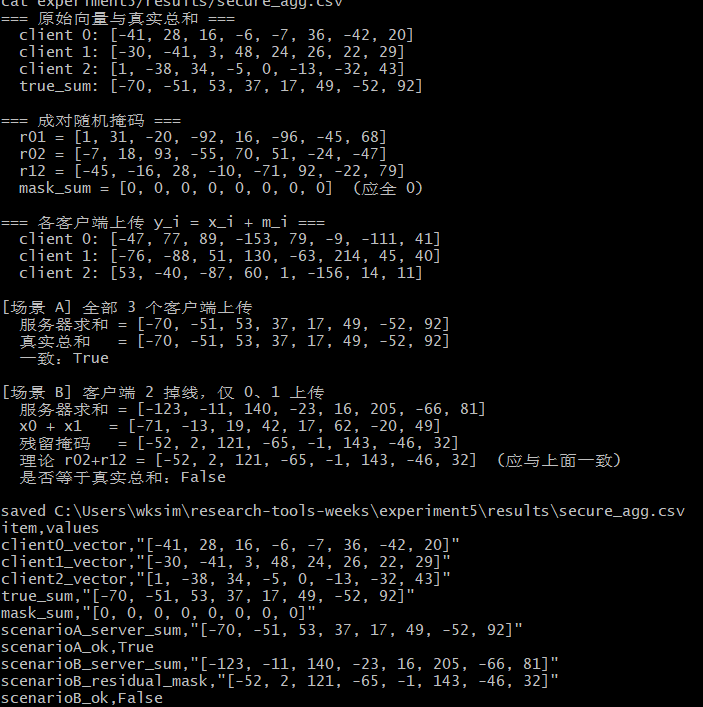
\includegraphics[width=0.92\textwidth]{figures/fig_secure_agg.png}
\caption{安全聚合演示输出（场景 A 掩码抵消得到真实和；场景 B 缺一客户端，残留掩码导致结果错误）}
\label{fig:secure-agg}
\end{figure}

\subsection{结果解释}

场景 A 中三个客户端的掩码两两成对、三项相加为零，服务器求和时掩码完全抵消，得到 $S$，且服务器全程未接触任何 $x_i$。以本次运行的第一个分量为例：$y_0 + y_1 + y_2 = -47 - 76 + 53 = -70$，与真实和 $-41 - 30 + 1 = -70$ 一致。

场景 B 中客户端 2 不上传，$m_2$ 缺失，剩下的 $m_0 + m_1 = r_{02} + r_{12}$ 无法抵消。本次运行中服务器求和为 $[-123, -11, 140, -23, 16, 205, -66, 81]$，残留掩码为 $[-52, 2, 121, -65, -1, 143, -46, 32]$，恰好等于 $r_{02} + r_{12}$，既不等于 $S$ 也不等于 $x_0 + x_1$。这说明\textbf{成对掩码机制依赖“全部客户端在线”这一前提}：任一客户端掉线，整个聚合结果就被污染。

\subsection{与完整安全聚合协议的区别}

本演示与 Bonawitz 等人提出的实用安全聚合协议（\cite{bonawitz2017practical}）有三点关键差异：

\begin{enumerate}
  \item \textbf{掉线恢复}：本演示假设所有客户端全程在线；完整协议用 Shamir 秘密共享把每个客户端的掩码分发给其他客户端，掉线时由存活客户端提交掩码分片，服务器可恢复掩码并剔除掉线者，得到剩余客户端的正确聚合。
  \item \textbf{防恶意客户端}：本演示假设客户端诚实，不主动伪造 $y_i$；完整协议加入双掩码（self-mask 与 pairwise-mask）与一致性校验，防止恶意客户端提交偏离值污染聚合。
  \item \textbf{密钥协商与身份认证}：本演示用固定种子本地生成掩码，不涉及真实的两两密钥协商与客户端身份认证；完整协议需要认证的 Diffie-Hellman 密钥协商，确保掩码只对协商双方可知。
\end{enumerate}

因此，本演示验证了成对掩码“相加为零、可抵消”的核心机制，但距离可部署的安全聚合还有掉线恢复、恶意安全与密钥管理三块工程内容。真实联邦学习系统（如 Flower 的 SecAgg 扩展）实现的是完整协议，不是这个简化版。

\section{实验总结}
\label{sec:optional}

本实验完成了联邦学习框架调研、MNIST 横向联邦图像分类复现与 Non-IID 对照：

\begin{enumerate}
  \item 选用 \textbf{Flower 1.43.0}，在 Windows 11 + Python 3.12 下用 Ray 模拟 1 个服务器与 5 个客户端，运行 FedAvg。
  \item 数据划分严格按题目要求：每类 500 张共 5000 张、seed=42，IID 每客户端每类 100，标签偏斜每客户端 2 类各 500；两套使用相同样本，验证脚本全部通过。
  \item 训练结果：IID 第 10 轮准确率 0.8799、损失 0.4736；标签偏斜第 10 轮 0.8129、0.8977。标签偏斜本地训练损失（0.1883）低于 IID（0.5025），但全局测试损失更高，体现 Non-IID 下的本地过拟合与全局泛化差距。
  \item 对照实验：5 个客户端各自独立训练 10 个 epoch，准确率 0.1853--0.2112、损失 5--7，远低于联邦标签偏斜模型（0.8129），证明参数聚合把分散类别信息汇集到全局模型的价值。
  \item 耗时：IID 50.29 s、标签偏斜 52.84 s，第 1 轮冷启动约 17 s，后续每轮 1.7--1.8 s。
  \item 隐私分析：本实验未启用安全聚合、同态加密或差分隐私；“数据不出本地”不等于隐私安全，参数上传仍可能泄露训练信息，保护思路包括安全聚合、差分隐私与同态加密。
  \item 拓展任务：实现 3 客户端成对随机掩码安全聚合演示，验证全参与时掩码抵消、缺一客户端时结果被残留掩码污染，并与完整安全聚合协议（Bonawitz 2017）的掉线恢复机制做对比。
\end{enumerate}

\textbf{选做任务完成说明：}本次完成了拓展任务——3 客户端整数向量求和的成对随机掩码安全聚合演示（第 \ref{sec:secure-agg} 节）。场景 A 中 3 个客户端全部上传，掩码两两抵消，服务器求和等于真实总和；场景 B 中客户端 2 掉线，残留掩码 $r_{02}+r_{12}$ 无法抵消，服务器求和被污染。演示验证了成对掩码的核心抵消机制，并说明了其与具备掉线恢复能力的完整安全聚合协议在掉线恢复、恶意安全、密钥协商三方面的差距。

% =========================================================
\bibliographystyle{plain}
\nocite{*}
\bibliography{reference}

\end{document}